%!TEX root = ../main.tex

\section{CAN bus}\label{sec:CANbus}
The CANOpen protocol runs on the CAN bus.
It was originally developed in the 1980's by Bosch.
It is a multi-master network, where each node connects to a common bus, and any node is then able to broadcast data to all other nodes.
The bus offers 1 Mbit/s on a bus up to 40 m of length. \todo{Martin: is this with or without the substantial overhead?}

\subsection{Physical Layer}\label{sub:CANphys}
The physical layer has three main parts: The CAN controller, the CAN transceiver and the bus itself. \\

The CAN controller can be implemented as a standalone IC, or in many cases integrated in the node itself.
The Zybo supports CAN, and an IP core is available, so the CAN controller is already given.\\

The CAN transceiver is connected to the controller by RX and TX voltage signals, and connects to the bus through two differential ports. 
The transceiver must support the standard ISO11898-2, as this is what the Sevcon motor driver uses.
The device SN65HVD232 from Texas instruments support this standard, and is supplied with 3.3 V, so it can be plugged right into the Zybo, and still communicate with the Sevcon even though its CAN bus uses $\si{5 \volt}$.
According to TI itself\cite{3.3V_CAN}, this family of $\si{3.3 \volt}$ transceivers are compatible and interoparable with other \si{5 \volt} transceivers, so long as they support the same standard.\\

The bus has to be made of twisted pair wires with a characteristic impedance of $\si{120 \ohm}$, and terminated at each end with a $\si{120 \ohm}$ resistor.
That means, that if the bus is broken at any point, no communication will work.
Alternately, it is possible to terminate each node, but this greatly reduces transmission speed, and will not be done.//

The transceivers have been mounted on boards, that plug directly into the Zybo's 12-pin PMOD connector, which will be stacked on top of each other. 
The scematic is showed below.

\begin{figure}[h!]
	\centering
	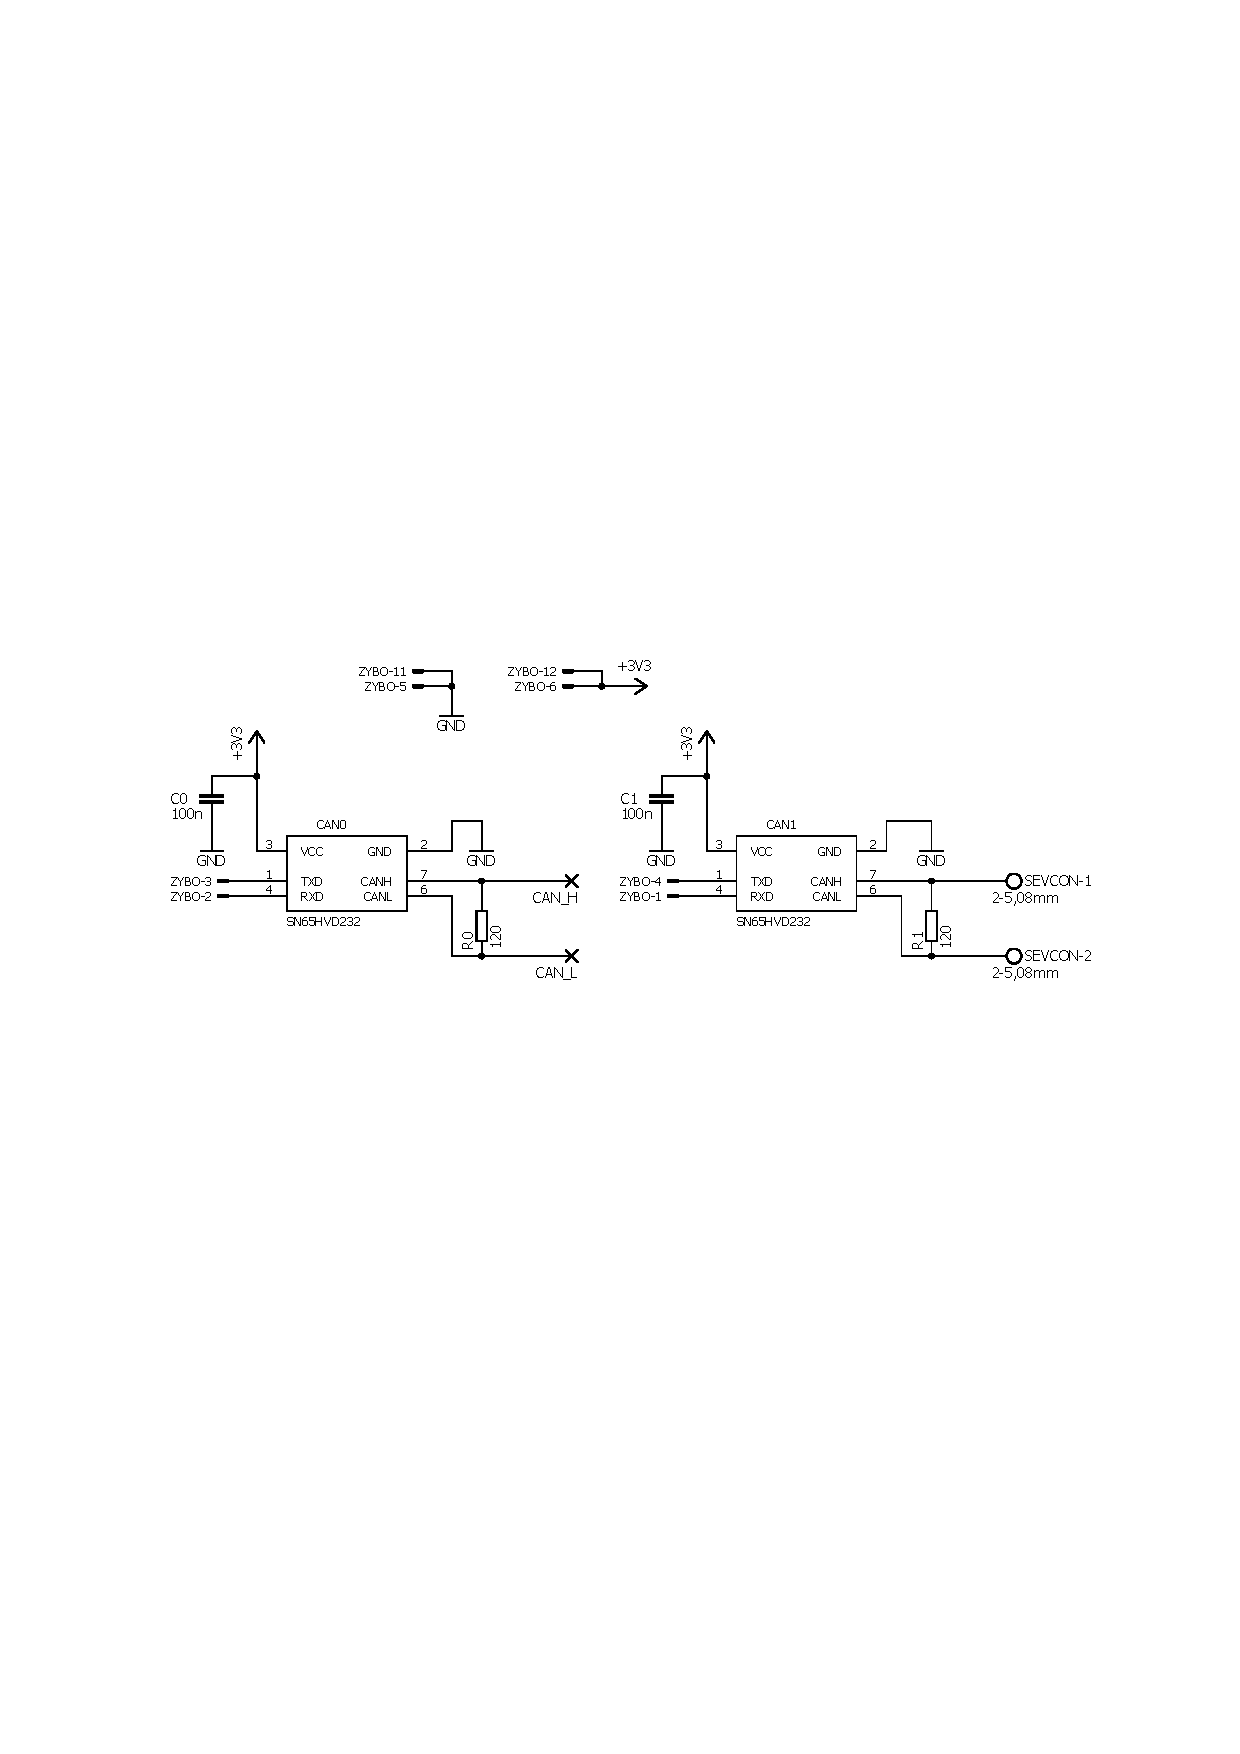
\includegraphics[width = 0.7\linewidth]{graphics/CAN_Schematic}
	\caption{Schematic of the two can transceivers. One board is build for two transceivers each with pads for termination}
	\label{fig:CAN_Schematic}
\end{figure}

The board has been designed to use the MIO ports, available in the PMOD JF. 
This is necessary to utilize the build in CAN controllers on the PS part of the Zybo.
Although the schematic contains two transceivers and two termination resistors, most of these devices are not mounted. 
Four boards will be made, all containing CAN0, C0 and the ZYBO connector. 
One board will also include the resistor R0 - this is the bottommost board
Another board will include R0, R1 CAN1, C1 and the SEVCON connector.
Ths is placed on top, to allow the SEVCON connector's screws to be accessible. 
The stack is visible below

\begin{figure}[H]
	\centering
	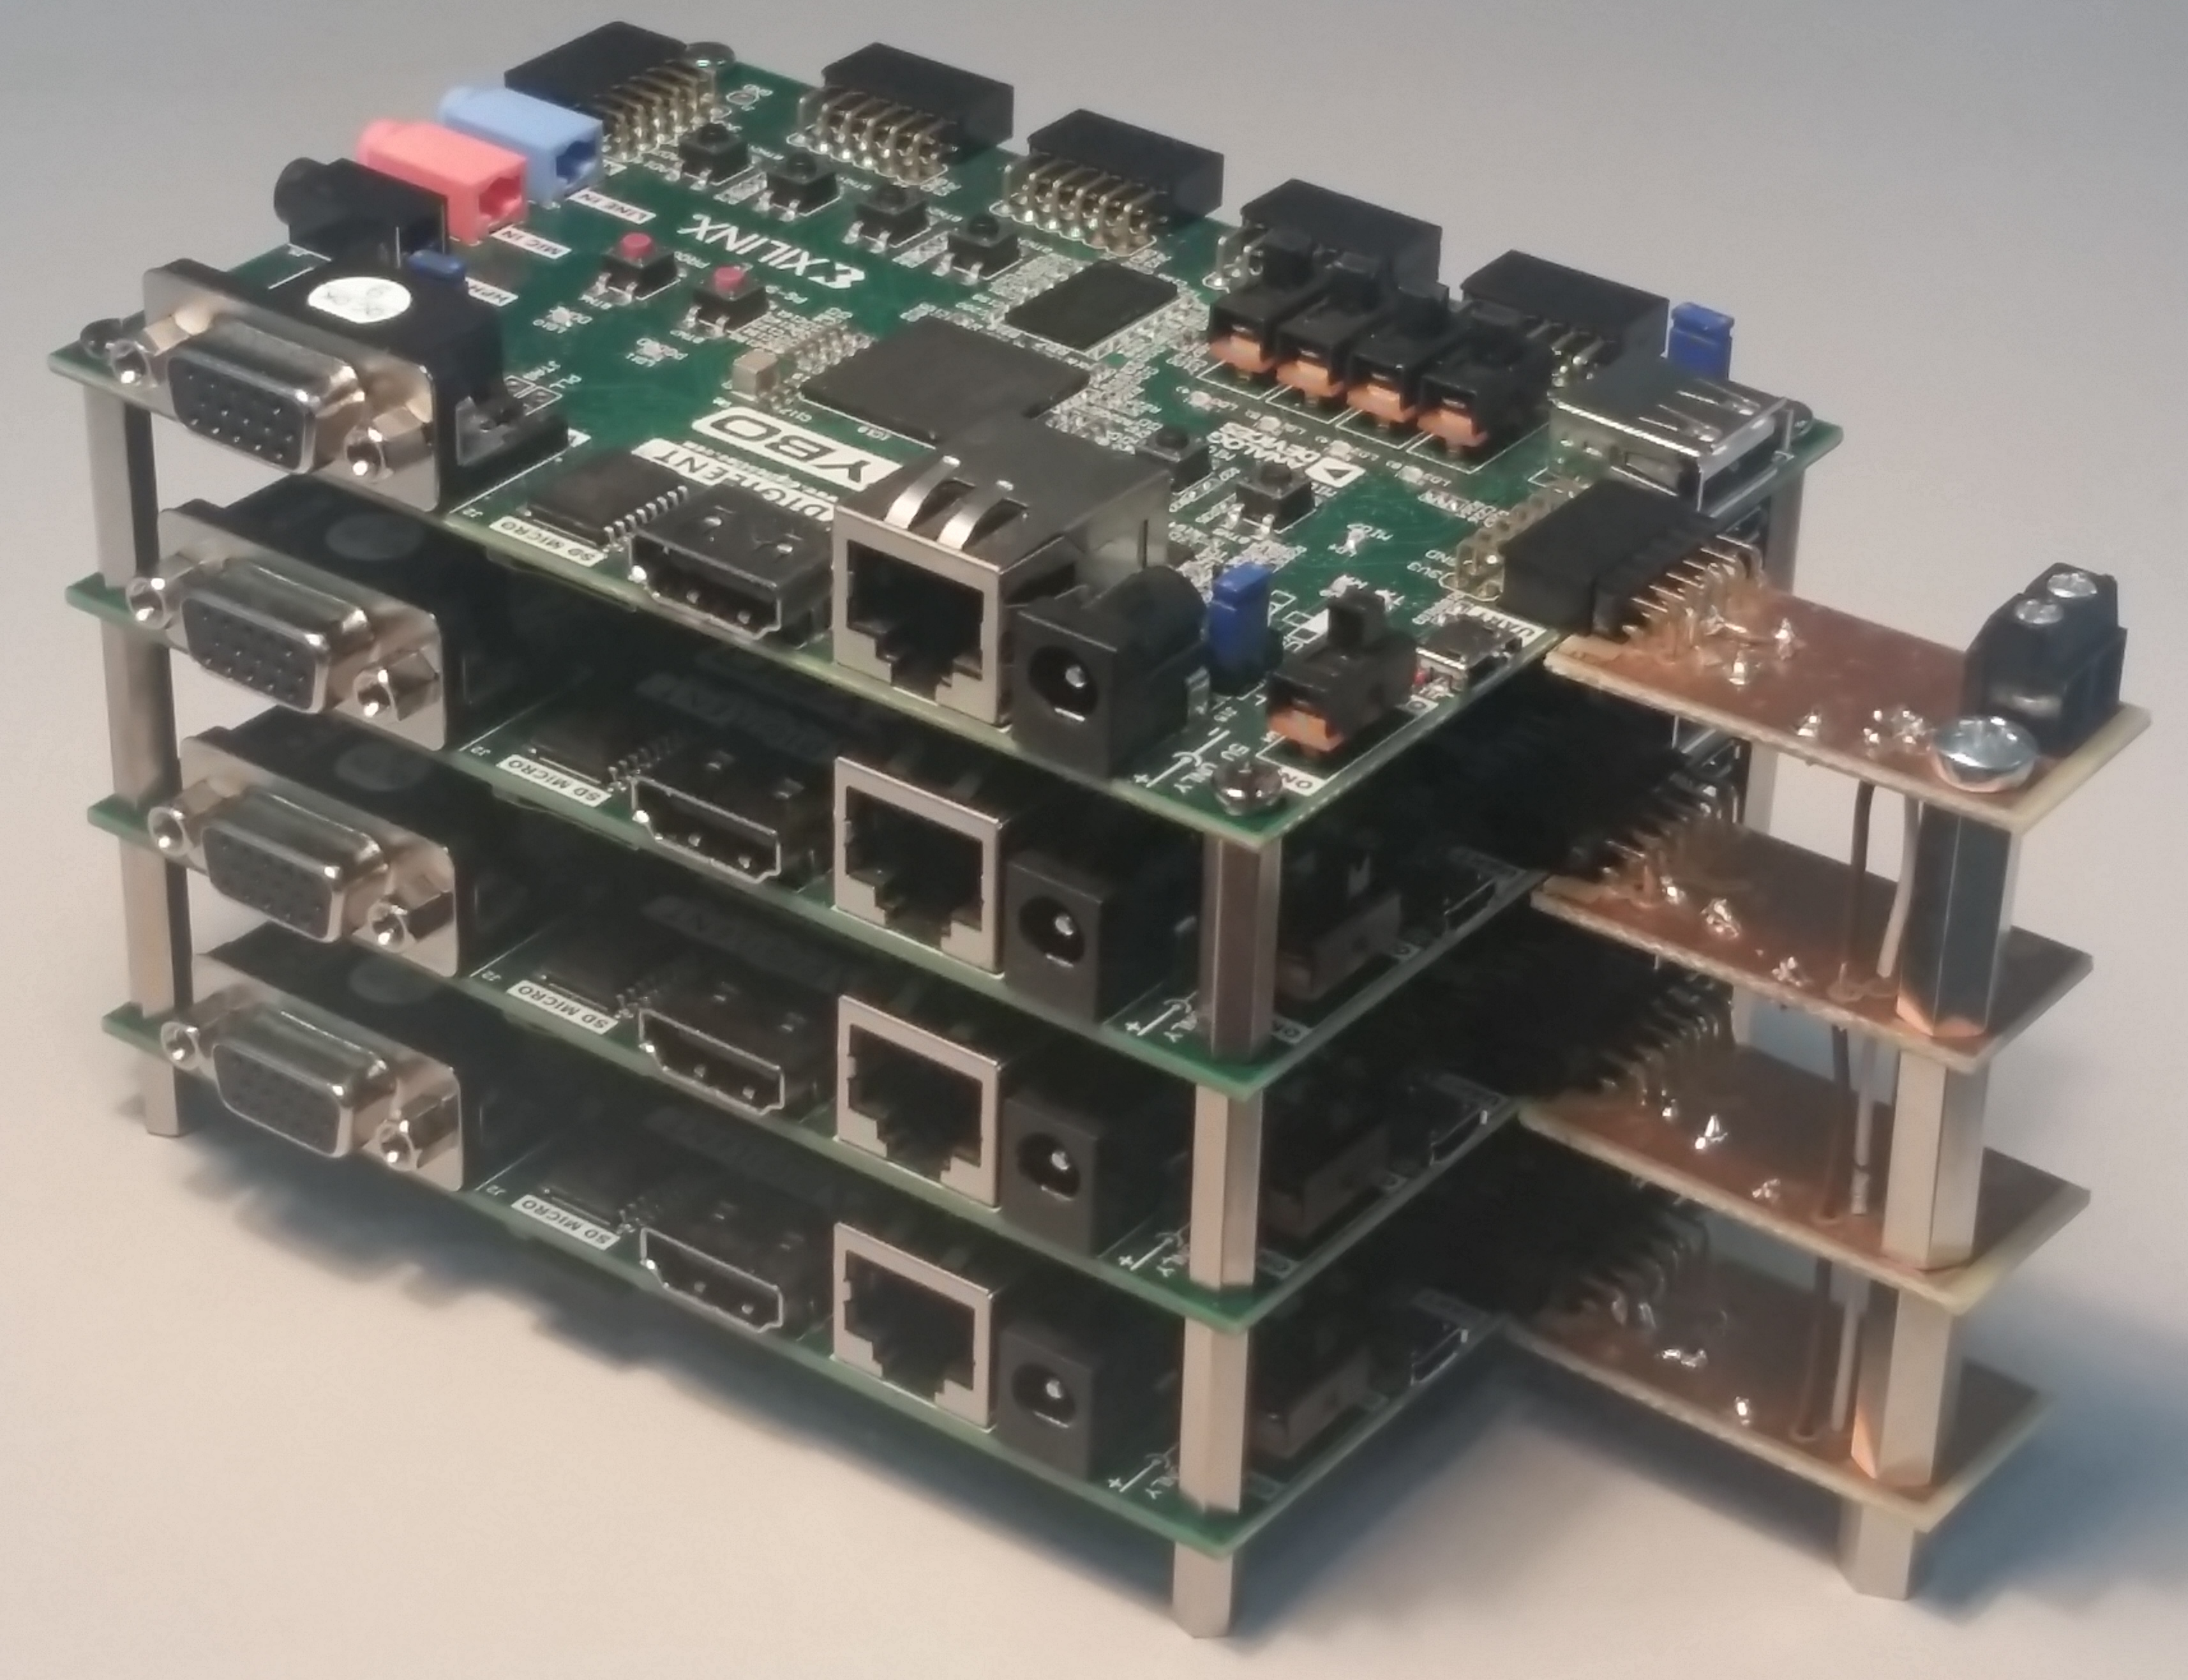
\includegraphics[width = 0.9\linewidth]{graphics/CAN_stack_picture}
	\caption{The CAN stack plugged into one Zybo}
	\label{fig:CAN_stack_picture}
\end{figure}

\subsection{Implementation of the Physical layer}\label{sub:CANphys_implementation}
The Zybo has two build in